\documentclass{jsarticle}

%
% プリアンブル
%
\usepackage{otf}
\usepackage[dvipdfmx]{graphicx}     % png 形式を利用するために付加

% 章立ての設定 
\renewcommand{\thesection}{第\arabic{section}章}

% 図表の設定
\makeatletter
  \def\thetable{\arabic{section}.\arabic{table}}
  \@addtoreset{table}{section}
  
  \def\thefigure{\arabic{section}.\arabic{figure}}
  \@addtoreset{figure}{section}
\makeatother

\begin{document}

\thispagestyle{empty}
\begin{center}
\Large
\textbf{2014年度 博士前期課程(ソフトウェア情報学) 論文}

\vspace*{23mm}
\Huge
\textbf{利用者の入力負荷軽減と推薦精度向上を図った観光推薦システムの構築と評価}

\vspace{5mm}

\LARGE
\textbf{Implementation and Evaluation of Sightseeing Spot Recommendation System Intend To Improve Precision and To Reduce Input Load}

\vspace{20mm}

\LARGE

岩手県立大学大学院 \\
ソフトウェア情報学研究科

\vspace{10mm}

2015年01月

\vspace{10mm}

2312013010

小松 一星

\vspace{18mm}

\begin{flushright}

\Large
研究指導教員\hspace{20mm}

\LARGE
\underline{\hspace{10mm}佐々木 淳\hspace{10mm}}

\underline{\hspace{10mm}菅原 光政\hspace{10mm}}

\underline{\hspace{10mm}阿部 昭博\hspace{10mm}}

% \vspace{3mm}
% \underline{\hspace{4.0cm}}
% 
% \vspace{3mm}
% \underline{\hspace{4.0cm}}
% 
% \vspace{3mm}
% \underline{\hspace{4.0cm}}

\end{flushright}


\end{center}

\newpage

\setcounter{page}{1}

\tableofcontents
\newpage
\listoftables
\newpage
\listoffigures
\newpage

\section{はじめに}

近年,我が国においては,若者の旅行離れが進んでおり,地域経済・文化の発展への悪影響が懸念されている.そこで我々は,旅行を促進する観光推薦システムを通じて若者と地域を結びつける仕組みの形成し,地域活性化へ寄与することを目指した.

本章では,本研究で対象とする観光の歴史と現状についてまとめ,今後の観光の発展に向けた課題について述べる.

\newpage

\subsection{観光促進の意義}

2013年,日本政府の閣僚によって構成される観光立国推進閣僚会議が立ち上げられた.本会議で決定された「観光立国実現に向けたアクション・プログラム2014\cite{action_program_2014}では観光について次のように述べている.

\begin{quote}
観光は,急速な成長を遂げるアジアをはじめとする世界の需要を取り込むことによって,日本の力強い経済を取り戻すための柱である.加えて,人口減少・少子高齢化が進展する中,国内外からの交流人口の拡大によって地域の活力を維持し,社会を発展させるとともに,諸外国との双方向の交流により,国際相互理解を深め,国際社会での日本の地位を確固たるものとするためにも,極めて重要な分野である.
\end{quote}

また,東日本大震災からの復興を新しい国づくりの契機にしたいとして2011年に発足した有識者らによる政策発信組織である日本創世会議においても,「地方元気戦略」のひとつに観光をキーワードとして挙げており,地方へ人を呼び込む魅力づくりの施策として期待されている\cite{nippon_sousei}.

さらに,経済面から観光を調査すると,世界全体GDPに占める観光関連業界のGDPは 9.1\% であり,金融業に次いで世界第2位の業種であることがわかる.
国内においても,その経済効果は大きい.我が国の観光統計の概要を図\ref{tourism_kibo}に示す.

\begin{figure}[!ht]
\begin{center}
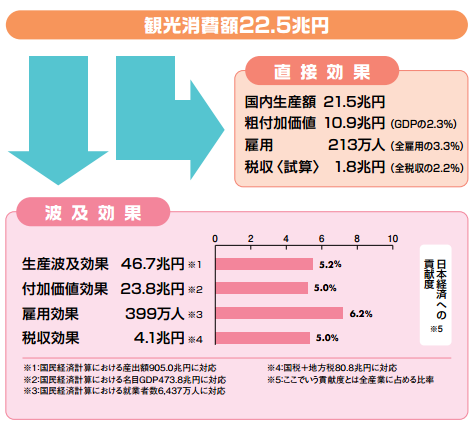
\includegraphics[width=9.0cm]{./image/tourism_kibo.png}
\caption{日本における観光統計の概要\cite{tourism_stat}}
\label{tourism_kibo}
\end{center}
\end{figure}

また,観光ビジネス研究会所属の中小企業診断士らによると,観光産業の発展を目指す理由を次のように挙げている\cite{tourism_future}.

\begin{enumerate}
\item 少子高齢化社会への対応: 国内需要の縮小が想定されるなか,我が国の伝統・文化・産業などのソフトパワーによる経済成長ができる可能性を持っている.
\item 地域経済の活性化: 地域独自の文化を含む観光資源を活用することで,国内外の旅行者との交流人口を増加させ,魅力的な地域を形成できる可能性を持っている.
\item 為替変動への対応: 観光産業は,原材料を必要としないため,安定的な経済社会の実現に向けた可能性を持っている.
\item 雇用の拡大: 若年層から熟年層まで幅広く雇用を生む可能性を持っている.
\end{enumerate}


以上のように,観光は国家戦略,経済戦略として重要な位置づけとされており,国内のみならず世界の地域文化・経済を支える分野である.したがって,観光促進に関する研究をする意義は大きい.

\subsection{観光分野の課題}

観光分野の発展はその波及効果も含めて大きな期待がされている.一方で,発展に向けた課題は数多くある.
観光行政を担当している観光庁が毎年発表している観光白書では,2010年から若者旅行の促進を課題のひとつとして毎年挙げている\cite{kanko_hakusho_2009}\cite{kanko_hakusho_2010}\cite{kanko_hakusho_2011}\cite{kanko_hakusho_2012}\cite{kanko_hakusho_2013}\cite{kanko_hakusho_2014}.観光白書では,若者の旅行離れが将来的な観光発展に大きな影響を与えることが危惧されている.この課題の解決に向けた有識者会議として2011年に若者旅行振興研究会が発足した.
本研究会では,発足にあたり次の課題を挙げている\cite{wakamono_shinko}.

\begin{enumerate}
\item 国内観光市場の低迷: 2005年以降,横ばいで推移しており,国内観光市場が発展していない
\item 日本人旅行の回数・宿泊数が減少傾向: 実質的に国内観光市場を支えている日本人旅行が低調.訪日外国人旅行は今後期待されているが,まだ市場は小さい.
\item 若者の旅行回数の減少: 20代・30代の旅行回数の落ち込みが顕著.他世代と比較して学生旅行の回数も大きく減少している.
\item 将来的に家族旅行の回数減少の懸念: 旅行回数の少ない若者がライフステージが変わったときに旅行行動をとらない可能性が高い.
\end{enumerate}

\subsection{推薦システムの発展}
\label{evolution_recommendation_system}

一方,情報工学分野では推薦システムの発展が近年著しい.推薦システムを簡潔に表現した定義は次のとおりである\cite{define_of_recommendation_system}.

\begin{quote}
どれに価値があるかを特定するのを助ける道具
\end{quote}

また,推薦システムが必要となった背景は2つある\cite{kamishima_recommendation}.

\begin{enumerate}
\item 大量の情報が発信されるようになった: 情報技術の進展により,容易かつ低コストで情報を発信できるようになった.
\item 誰もが大量の情報を取得できるようになった: 情報を参照できる状態だが,それを識別できない状況が生じた.(情報過多\cite{information_overload})
\end{enumerate}

これらの背景もあり,推薦システムの研究は進み,産業界においても利活用によって業績を伸ばす事例が出ており,最近では,Webを通じた各種サービスの機能で活用されている.
推薦システムを活用した情報サービスの例を以下に挙げる.

\begin{enumerate}
\item Amazon\cite{amazon}: 書籍の情報推薦を行う.購入を検討している書籍に関連する書籍をおすすめとして提示したり,これまで購入した書籍に関連する書籍を推薦する.
\item Gunosy\cite{gunosy}: ニュース記事の情報推薦を行う.利用者個人の興味のある分野を推定し,その内容に応じてニュースを推薦する.
\item オンライン広告\cite{yahoo_ad}\cite{facebook_ad}\cite{google_ad}: 購買行動を促進する効果的な広告を表示する.利用者のWebサイト利用状況や過去に興味を持った広告などの情報を活用して広告を推薦する.
\end{enumerate}

以上のように,情報工学分野では推薦システムの研究が進み,産業界においても利用され,情報過多の時代とされる現代において人々の生活を助ける道具として活躍している.

\subsection{本研究の目的}

これまでの説明によって,観光は我が国のみならず世界全体として主要な産業のひとつであり,我が国の成長にとっても重要な分野であることが明らかになった.観光庁は,観光分野の発展に向けて,若者旅行の促進を政策のひとつとあげており,若者旅行振興研究会を発足させた.本研究会では, 若者旅行振興のための課題を示している.

一方,情報工学分野においては新しい情報発信の仕組みとして推薦システムの実践利用が進んでいる.我々は,観光領域に情報推薦の仕組みを適用し,消費者の行動データをもとにしたパーソナライズした地域情報発信を行い,行動データの観光推薦への活用可能性を検証することを目的として研究を進めることとした.本研究によって観光分野の発展および地域活性化に寄与することを狙う.

\subsection{本論文の構成}

本論文は,6章から構成される.
第1章では,本研究の概観として,観光の現状と推薦システムの現状を示した.
第2章では,本研究で扱う観光領域について調査し,本研究における観光の位置づけを述べる.
第3章では,観光領域での推薦システムの活用事例について調査し,本研究で解決を目指す具体的な課題を明らかにする.
第4章では,課題解決を図った観光推薦システムの提案・設計を示す.
第5章では,開発したプロトタイプシステムの運用結果とその評価を質的観点と量的観点からまとめ,考察する.
第6章では,本研究のまとめと今後の課題について述べる.

\subsection{本章のまとめ}

本章では,観光分野の研究を実施する意義を明らかにし,本研究の目的を,行動データの観光推薦への活用可能性の検証であることを示した.
次章以降では,既存研究,関連事例などを細かに調査し,その解決を図る.

\newpage

\section{観光の概観}

本章では,本研究で扱う観光領域について調査し,本研究における観光の位置づけを述べることを目的とする.

本章は,5節で構成される.\ref{history_of_tourism}節では,観光の歴史を語源から調査した内容を述べる.\ref{history_of_tourism_study}節では,観光学とその周辺研究の歴史を各種学会とともにまとめる.\ref{definition_of_tourism}節では,歴史的背景,学問的背景から観光の定義について調べた内容をまとめる.2.4節では,観光に関連する関連用語の定義について述べたのちに本論文で論ずる観光の定義を示す.2.5節では,観光の概観をまとめる.

\newpage

\subsection{観光の語源}

\label{history_of_tourism}

観光という言葉は,中国の「益経」という書物のなかの「国の光を観る.用て王の賓たるに利し」という一節によるとされている\cite{kanko_define}.
ここでいう「国の光」とは,国王の人徳と善政によって国が反映し,その国を訪れる人々にはその国が光に輝いて見えることをいう.すなわち,観光とは,その「国の光」を観ることである.

\subsection{観光研究の歴史}

\label{history_of_tourism_study}

一般に,観光は余暇の時間に実施する人間の行為であり,観光を実施するには金銭的な支出が必要であるとされている.我が国においての観光は,経済的に豊かになった高度経済成長期から盛んに注目され,これまで一部の富裕層にのみが実施できた観光が多くの国民にとって身近なものになった.
それに伴い,観光の学問的な取り組みのニーズが高まり,我が国では1960年に日本観光学会が設立され,観光研究が始まった.日本国内の主な学会を 表\ref{japanese_society} に示す.


\begin{table}[!h]
\small
\caption{日本国内の主な学会\cite{japanese_society_list}}
\begin{center}
\begin{tabular}{lll}
\label{japanese_society}
学会名 & 設立年 & 活動目的 \\ \hline
日本観光学会                            & 1960年 & 観光及び観光事業に関する学術の進歩・普及\cite{society_tourism}  \\
日本ホスピタリティ・マネジメント学会    & 1992年 & ホスピタリティの考え方を基軸としたマネジメント研究\cite{society_hm}  \\
日本国際観光学会                        & 1993年 & 国際観光の学術研究の推進\cite{society_jafit} \\
余暇ツーリズム学会                      & 2001年 & 余暇領域の研究\cite{society_yoka} \\
総合観光学会                            & 2001年 & 専門分野を超えた総合観光学の確立と観光地域の持続的な発展\cite{society_afz} \\
観光まちづくり学会                      & 2001年 & 観光をまちづくりの視点で研究\cite{society_m}  \\
日本観光ホスピタリティ教育学会          & 2002年 & 観光とホスピタリティに関わる教育の在り方を探究する\cite{society_jsthe}  \\
観光情報学会                            & 2003年 & 観光学と情報科学技術に関する学術的視点と観光産業の融合\cite{society_sti}  \\
長崎国際大学 国際観光学会               & 2005年 & 長崎国際大学での研究成果を公開し広く情報交換を得ること\cite{society_niu}  \\
日豪ツーリズム学会                      & 2007年 & 日豪観光分野における交流の促進に関して調査・研究\cite{society_jatf} \\
国際観光医療学会                        & 2010年 & 観光と医療に携わる領域の研究ならびに交流\cite{society_iatm}  \\
日中国際ツーリズム学会                  & 2010年 & 中日ツーリズムの国際協力に関する研究\cite{society_duan}  \\
コンテンツツーリズム学会                & 2011年 & コンテンツを活用した観光振興及び地域活性化の研究と実践\cite{society_ct}  \\
観光学術学会                            & 2012年 & 観光学の学術的発展と普及\cite{society_jsts}  \\
\end{tabular}
\end{center}
\end{table}


\subsection{観光の定義}

\label{definition_of_tourism}

観光学は,いまだ発展途上の学問であり,現時点で「観光」の普遍的な定義を示すのは難しいとされている\cite{kanko_define}.
観光の定義には,代表的なものがいくつかあるが,研究の必要により研究者によっては独自の定義を用いる場合も多い.

ここでは代表的な定義を示したうえで,本研究での定義を述べる.


\subsubsection{経済学としての観光定義}

観光は,経済学者が「見えざる輸出」(invisible export) として重要性に注目したことによって始まったとされている\cite{kanko_define}.最初の研究課題は,その経済効果をどのように測定するかである.オギルヴィエは,観光の本質が「一時的滞在地において他所で取得した収入を消費すること」と定義した\cite{tourism_economy1}.一方,グリュックスマンは,「ある土地における一時的滞在者とその土地の住民との間の諸般の関係」と考えた\cite{tourism_economy2}.

\subsubsection{一般的な定義としての観光}

特定の研究目的を念頭におかず,一般的な定義として代表的に利用されたのは,井上による「人が日常生活圏を離れて,再び戻る予定で,レクリエーションを求めて移動すること」である\cite{inoue}.

\subsubsection{国際的な定義}

世界観光機構(WTO: World Tourism Organization) では,「訪問の主要な目的が,訪問国内で報酬を得るための活動を行うこと以外の者で,1泊以上12ヶ月を超えない期間,居住国以外の国で通常の生活環境を離れて旅行する人」としている\cite{wto}.

\subsection{観光関連用語の定義}

これまで「観光」は,普遍的な定義がなく,観光を扱う者によってその定義が異なることを示した.ここでは同様に,観光に関連する用語の定義を概観として示す.

\subsubsection{観光対象}

観光という行動には,なんらかの対象がある.それを観光対象と呼ぶ\cite{yokomizo_1998}.
観光対象は階層構造で表すことができる.その構造を図\ref{tourism_type}に示す.


\begin{figure}[!ht]
\begin{center}
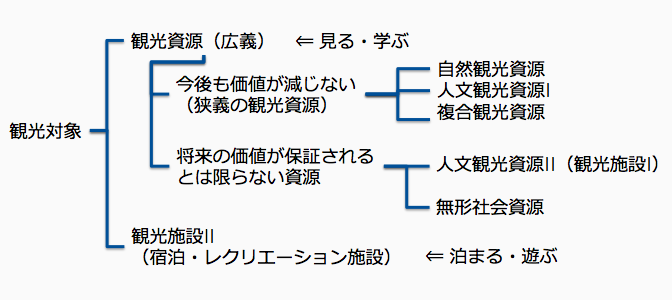
\includegraphics[width=8.0cm]{./image/tourism_type.png}
\caption{観光対象の構造}
\label{tourism_type}
\end{center}
\end{figure}



観光対象は2つの要素で構成されている.1つ目は,観光資源である.2つ目は,観光施設IIである.その言葉の定義を次小節にて示す.

\subsubsection{観光資源}

観光資源という言葉には,広義の定義と狭義の定義が存在する.
まず狭義の観光資源とは,「今後とも価値が減じない資源」であり,長い時間の経過を経て,価値がでた資源である.これには,人間が創造することのできない自然観光資源と先人が長い時間を経て価値を創造した人文観光資源I,およびこれら2種を融合した複合観光資源の3つで構成されている.

一方,広義の観光資源は,狭義の観光資源のほかに,将来の価値が保証されるとは限らない資源のうち,人工観光資源(観光施設I)もしくは無形社会資源を含んだもの指す.例を挙げると,前者は年間数百万人が来場するテーマパークなど,後者は文化的側面の強い風俗・衣食住・芸術・言語などである.

観光学上の観光資源は,いわゆる「見る・学ぶ」に相当する.

\subsubsection{観光施設II}

観光施設IIは,宿泊施設やレクリエーション施設である.この区分にある対象は,将来的に長い時間を経て,観光施設Iの区分に移動する可能性がある.
観光学上の観光施設IIは,いわゆる「泊まる・遊ぶ」に相当する.


\subsubsection{公的な用語の定義}

これまでは観光学の側面から体系だてられた区分を紹介した.ここでは,政府・官公庁が利用する公的な定義をまとめて紹介する.

\begin{enumerate}
\item 観光      : 余暇の時間の中で,日常生活圏を離れて行う様々な活動であって,触れあい,学び,遊ぶということを目的とするもの\cite{toshin_1995}.
\item 観光資源  : 史跡,名勝,天然記念物等の文化財,歴史的風土,優れた自然の風景地,良好な景観,温泉その他文化,産業等に関するもの\cite{tourism_law_2007}.
\item 観光地    : 観光資源の集積及び地域的なまとまり\cite{tourism_kensetsu_1974}.
\item 観光地域  : 観光地の集積,一日周遊圏\cite{tourism_kensetsu_1974}.
\end{enumerate}

\subsubsection{本研究で用いる用語の定義}

これまで観光と観光に関わる用語を調査を行ったが,その言葉の定義は確立されたものではない.しかし,研究を進めるにあたり,用語を定義する必要がある.そこで我々は,公的な定義を中心に一般的な定義を決定した.また,情報工学上での観光情報の扱いに関しては明確な定義に沿うデータ取り扱いは難しい.そこで,一般的な定義を包含する広義の定義を用いて論じていくこととした.これらをまとめたものを表\ref{define_of_tourism}に示す.

\begin{table}[!h]
\small
\caption{本研究における用語の定義}
\begin{center}
\begin{tabular}{lp{30zw}p{15zw}}
\label{define_of_tourism}
用語 & 一般的な定義 & 本研究での定義 \\ \hline
観光        & 余暇の時間の中で,日常生活圏を離れて行う様々な活動であって,触れあい,学び,遊ぶということを目的とするもの        & 移動を伴う様々な活動 \\
観光資源    & 史跡,名勝,天然記念物等の文化財,歴史的風土,優れた自然の風景地,良好な景観,温泉その他文化,産業等に関するもの  & 移動を伴う様々な活動の目的地もしくは経由地 \\
観光地      & 観光資源の集積及び地域的なまとまり    & 地域的なまとまり(市区町村) \\
観光地域    & 観光地の集積.一日周遊圏              & 観光地の集積(都道府県) \\
観光推薦    & --                                    & なんらかの情報に基づいて,観光資源,観光地,観光地域などを推薦し,旅行者に価値のある情報を届けること
\end{tabular}
\end{center}
\end{table}

\subsection{本章のまとめ}

本章では,本研究で扱う観光領域について調査した内容をまとめた.観光の語源は「(国の)光を観る」行為であり,もともと日本においては一般的に実施されるものではなかった.しかし,戦後の経済成長ともに観光が多くの国民において身近になることに伴い,学会が設立され国内における観光研究がはじまった.学問としての観光の定義は定まっていない.そこで本研究で論ずる言葉の定義を示した.

\newpage

\section{既存研究・関連事例}

本章では,推薦システムの現状と観光推薦システムの既存研究および関連事例についてまとめ,本研究によって解決を目指す課題について明らかにする.

本章は,4節で構成される.3.1節では,推薦システムの概要を述べる.現状の推薦システムの研究において十分に発達した事柄について扱う.3.2節では,推薦システムを観光領域に適用した事例を紹介し,それぞれの事例の課題を述べる.3.3節では,本研究で解決を目指す課題を明らかにする.3.4節では,既存研究と関連事例に触れたのちに本章をまとめる.

\newpage
\subsection{推薦システムの概要}

\ref{evolution_recommendation_system} 節では,推薦システムの発展について簡単に紹介した.ここでは,これまで研究が十分に発達した事柄について詳しく紹介し,次節以降の既存の観光推薦システムの事例につなげる.

\subsubsection{推薦の度合い}

推薦システムは,なんらかのアルゴリズムでアイテム(商品などの推薦される対象)を推薦する.この推薦には,個人化の度合いが3つあるとされている\cite{define_of_recommendation_system}\cite{recommendation_type_of_personalize}.

\begin{description}
\item[非個人化推薦] すべての利用者について同じ推薦を行う.いわゆる人気ランキングや新着ランキングなどである.単純な集計関数(合計,平均など)を用いて推薦アイテムを決定するため,実装が容易なことが特徴である.
\item[一時個人化推薦] 利用者の利用の単位(セッション)で,同じ入力や振る舞いをした利用者に同じ推薦を行う.例えば,あるアイテムに関する評価や詳細情報を付加することもこの区分の一種である.別例としては,検索の絞り込みや占い診断のように一定の条件化において同じ推薦を行うものはこの一例になると考えられる.
\item[永続的個人化推薦] 利用者の個人情報や過去の行動情報に応じて,異なる推薦をするものである.例えば,利用者による過去に購入したあるアイテムに関する評価情報に基づいて,関心があるであろう別のアイテムを推薦することである.
\end{description}

本論文では,特に断りのない限り永続的個人化推薦を「推薦」という言葉として取り扱うことにする.

\subsubsection{推薦アルゴリズムの分類}

推薦を行うには,システムが利用者について何らかの情報(以下,ユーザプロファイルという)を知っている必要がある.
ここでは,ユーザプロファイルを用いて推薦をするためのアルゴリズムとして近年よく利用される代表的な4つアプローチを述べる.

\begin{description}
\item[協調型] 協調型推薦のアプローチは,既存のユーザコミュニティの過去の振る舞いや意見を用いて,システムを利用する対象のユーザの好みやおそらく興味を持つであろう情報を予測し,発掘することである.
\item[内容ベース型] 内容ベース型のアプローチは,アイテムの特徴やユーザの好みなど,推薦対象の内容を考慮してアイテムを推薦する手法である.
\item[知識ベース型] ユーザの要求とアイテムの類似性,もしくは明示的な推薦ルールに基づいて推薦する手法である.
\item[ハイブリッド型] これまで説明した3つのアプローチを組み合わせて利用する手法である.
\end{description}

\subsubsection{推薦システムの評価}

推薦システムの研究においては,推薦の質を向上させることは重要である.質の向上を図るには質を比較する指標が必要である.
ここでは,推薦システムの評価に用いられる主要な指標を述べる.

\begin{description}
\item[適合率(Precision)] 推薦アイテム群のうち,正しく推薦したアイテム群の割合
\item[再現率(Recall)]  正解とされるアイテム群(テストデータ)のうち,正しく推薦したアイテム群の割合
\item[f値]  一般に適合率と再現率はトレードオフの関係になるため,総合的に比較できる指標を算出する目的でよく用いられるもの.変数として適合率と再現率を用いており,適合率と再現率の低い方の値に偏って平均をとる.
\end{description}

\subsection{観光推薦システムの必要性と関連研究事例}

前節では,推薦システムの概要を示した.ここでは,観光領域における推薦システムの研究および関連事例をそれぞれの研究の課題ともに明らかにする.

\subsubsection{協調フィルタリングとコンテンツ分析を利用した観光地推薦手法の提案}

樽井らの研究\cite{tarui}では,協調フィルタリングの利点とコンテンツ分析法の利点を組み合わせた観光地推薦手法を提案している.
観光推薦のアプローチとしては,まず次の3つのベクトルを算出する.

\begin{description}
\item[観光地特徴ベクトル] 観光地の特徴を最もよく表している観光特性を要素に持つベクトル
\item[利用者履歴ベクトル] 利用者の旅行履歴を要素に持つベクトル
\item[利用者特徴ベクトル] 利用者が旅行先の選定に重視してきた観光特性を要素に持つベクトル
\end{description}

次に,これらのベクトルを入力値とした協調フィルタリングを実施し,観光地(本論文の定義でいう「観光資源」)を推薦する.
著者はこの研究の課題として,「観光地推薦アルゴリズムの妥当性の検証と利用者テストの実施」を挙げている.
また,利用者履歴ベクトルの入力は,これまで訪れたことのある観光地をすべて入力する必要があり実用的ではないと考える.

\subsubsection{旅行プラン作成支援ツールCT-Planner}

倉田らの研究\cite{ctplanner}\cite{ctplanner2}\cite{ctplanner3}\cite{ctplanner3b}\cite{ctplanner4}\cite{ctplanner5} では,Web上で対話的に旅行プランの作成ができるツール「CT-Planner\cite{ctplanner_web}」を開発している.
本システムは,利用者の要望をレーダーチャートなどで入力し,対話的に旅行プラン(観光ルート; 観光資源の順列)を推薦するものである.

本システムの評価は,ユーザに対してのアンケート・インタビューによるもの主であるが,これまでのユーザの観光実績に基づく推薦精度の視点では評価をしていない.

\subsection{本研究で解決を目指す課題}
\label{problem}

前節では,これまでの観光推薦システムの研究がどこまで進められているかについて概観した.
現在の観光推薦システムは下記の課題があることがわかった.

\begin{description}
\item[観光行動に関するデータセットが見当たらない(データセットの問題)]
       データセットとは,プログラムが処理をするデータの単位であり,ここでは推薦アルゴリズムの実験・改良などに利用するためのものを指す.情報推薦領域では多くの研究が行われているが,観光に関するデータセットは存在せず,観光推薦の研究を進めるうえで障害となっている.
\item[観光行動の入力に手間がかかる(行動データ入力の問題)]
       これまでの観光行動を利用者の特性として観光推薦に利用するアプローチは見られる.しかし,入力には手間がかかることが想定される.
\item[観光推薦領域において実データを利用した評価を行っている研究は見当たらない(行動データの定量評価問題)]
       推薦システムにおいて利用される評価アプローチとして,正解データの一部をマスクしたうえで該当データを推薦システムがどれだけ推薦できたかを評価するものがある.観光推薦システムの領域ではこの方法を利用して推薦精度を評価した事例が見当たらない.
\end{description}

本研究では,以上の3つの課題点を解決する提案を次章以降で述べていく.

\subsection{本章のまとめ}

本章では,推薦システムの現状と観光推薦システムの既存研究および関連事例についてまとめ,本研究によって解決を目指す課題について明らかにした. 

\newpage

\section{提案}

本章では,前章までに明らかになった研究の課題を解決するシステムの要件定義,設計,開発を行った経過を示す.

本章は,5節で構成される.4.1節では,課題を解決するために必要なシステム要件を定義する.4.2節では,要件を満たすために活用するチェックインサービスと汎用的な機械学習ライブラリ「Apache Mahout」について概観を説明する.4.3節では,システム設計として,概要図,システム構成図,データベース設計,API設計,バッチ設計および動作環境を提示する.4.4節では,開発したシステムの画面例を機能とともに紹介する.4.5節では,提案システムの設計・開発について総括し本章のまとめとする.

\newpage
\subsection{システム要件}

\ref{problem} 節で明らかになった3つ課題の解決を満たすシステムとして,3つのシステム要件を掲げた.

\begin{enumerate}
\item データセット保管要件: 推薦アルゴリズム改良のために観光行動データセットを保管すること
\item 観光行動自動取得要件: 利用者に手間をかけずに過去の観光行動を取得できること
\item 観光推薦・評価要件: 実データを利用した推薦を実施し精度を評価すること
\end{enumerate}



なお,上記の要件を満たす推薦システムを開発することによって,今後の観光推薦研究のためのデータ収集・評価サイクルが副次的につくられる.

\subsection{利用する外部サービスとライブラリ}

掲げられた要件を満たすシステムを提案するにあたり,利用するサービスおよびライブラリについて説明する.

\subsubsection{チェックインサービス}

チェックインサービスとは,ソーシャルネットワーキングサービス(以下,SNS)の一種である.SNSと同様にユーザは利用登録を行い,サービス内に友人ネットワーク関係を構築し,自身に関する情報を発信することができる.特にチェックインサービスにおいては,自分がいる場所もしくは自分がいた場所を友人に対して発信する(チェックイン)ことで友人とコミュニケーションするサービスである.

代表的なサービスとしては,Foursquare\cite{foursquare}(2014年5月に swarm という名称に変更された)およびFacebook\cite{facebook}がある.それぞれの特徴を表\ref{features_of_checkin_service}に示す.

\begin{table}[!h]
\small
\caption{主要なチェックインサービスと特徴}
\begin{center}
\begin{tabular}{lll}
\label{features_of_checkin_service}
特徴\サービス名            & Foursquare                    & Facebook \\ \hline
利用者数(世界)            & 4500万人                      & 13億人 \\
蓄積されている主なデータ    & 誰が,いつ,どこに行ったか    & 利用者プロフィール,誰が,いつ,どこに行ったか \\
第三者利用の仕組み          & あり                          & あり \\
時価総額                    & 約80億円(非上場)            & 約19兆円 \\
\end{tabular}
\end{center}
\end{table}

どのチェックインサービスも類似した機能を有しており,利用者数も多く日常的にサービスを利用している人も少なくない.
加えて,第三者利用の仕組みがある.第三者利用の仕組みとは,利用者の個別の許可を得られれば,チェックインサービスの運営会社以外の第三者に対して,これまで蓄積した個人のチェックインデータを連携することができる仕組みである.

これらの特徴を踏まえると,要件を満たすシステムを開発するにあたり,チェックインサービスのデータを活用することが相応しいと考えた.

\subsubsection{Apache Mahout}

Apache Mahout は,Apache Software Foundation が開発を進めるオープンソースの機械学習ライブラリである\cite{mahout}.大きく分けて,「レコメンデーション」「クラスタリング」「分類」の領域の機械学習が実装されている.Apache Software Foundation のトップレベルプロジェクトのひとつであり現在も開発が活発で,同組織が開発する大規模データ処理基盤 Apache Hadoop などとの連携も行われている.

これらの特徴を踏まえると,要件を満たすシステムを開発するにあたり,このライブラリを利用することによって容易に推薦システムの仕組みを整えられると考えた.

なお,本論文では,効果的な推薦アルゴリズムの選定は主題ではないため,チェックインデータを利用して容易に推薦ができる協調フィルタリングを利用することとした.

\subsection{システム設計}

これまで紹介したチェックインサービスおよび Apache Mahout を用いて観光推薦システムのプロトタイプを設計した.
本システムは2つのモジュールで構成されている.1つは,特徴収集モジュールである.このモジュールでは,利用者からチェックインサービスの第三者利用の承認を得たうえで,チェックインサービス上にあるデータを収集し,システムのデータベースに格納する.もう一方のモジュールは,推薦モジュールである.本モジュールでは,蓄積されたチェックインデータを活用して観光推薦を実施する.

推薦アルゴリズムは,次に3つのパターンを入力値として協調フィルタリング(アイテムベース,コサイン類似度)に基づいて観光推薦を行う.

\begin{description}
\item[観光地域推薦(都道府県推薦)] 利用者のチェックインデータを都道府県の単位に名寄せさせたものを入力値としたもの.
\item[観光地推薦(市区町村推薦)] 利用者のチェックインデータを市区町村の単位に名寄せさせたものを入力値としたもの.
\item[観光資源推薦(スポット推薦)] 利用者のチェックインデータをそのまま入力値としたもの.
\end{description}


それぞれのパターンともに,アイテム(都道府県,市区町村および観光資源のいずれか)とユーザの行列を入力値とする.行列の値は,行ったことがあれば1, 行ったことがなければ0となる.

\subsubsection{システム概要図}

提案システムのシステム概要図を図\ref{system2}に示す.特徴収集モジュールが実施する流れ 1〜3 によって,「観光行動自動取得要件」を満たすことができる.また,流れ 4〜6 によって,「観光推薦・評価要件」を満たすことができる.

\begin{figure}[!ht]
\begin{center}
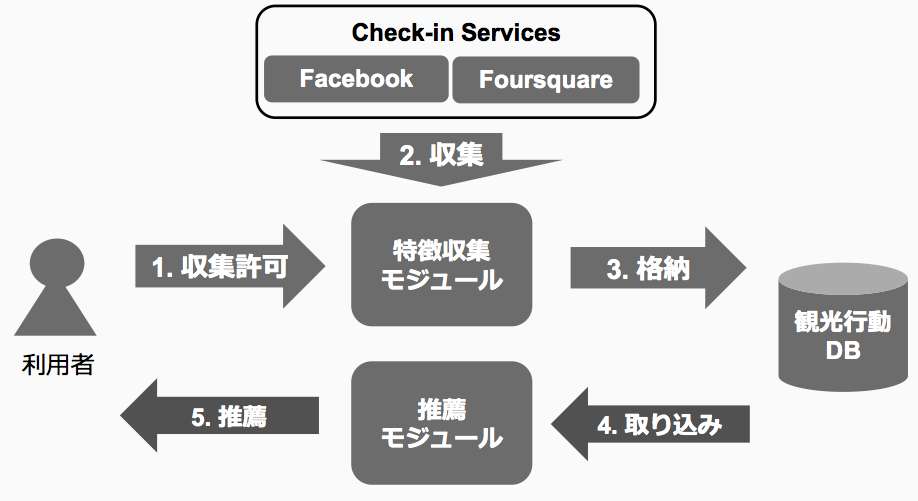
\includegraphics[width=12.0cm]{./image/system2.png}
\caption{システム概要図}
\label{system2}
\end{center}
\end{figure}

\subsubsection{システム構成図}

提案システムのシステム構成図を図\ref{system1}に示す.より具体的な設計は後述するが,本システムは,一般的なWebアーキテクチャに従って構築されている.

\begin{figure}[!ht]
\begin{center}
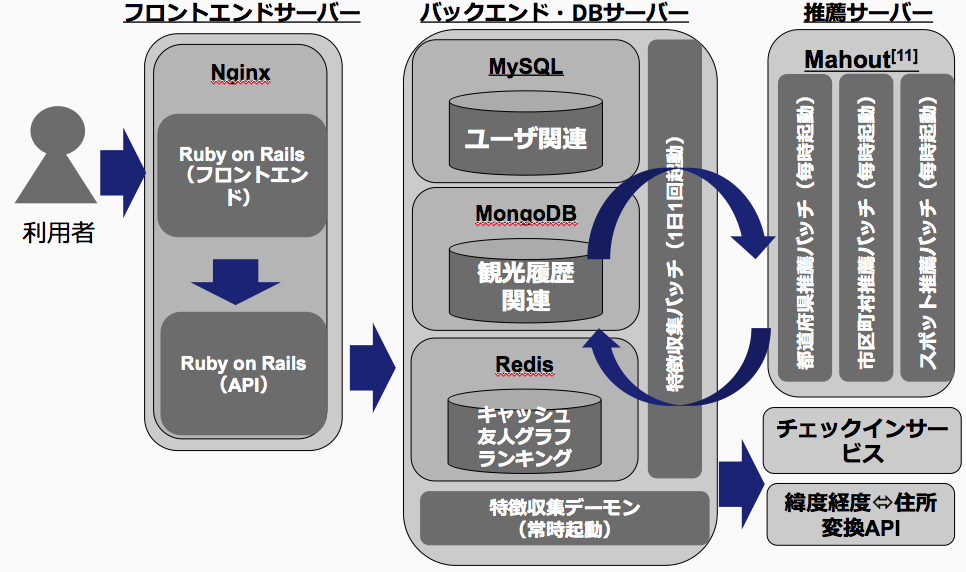
\includegraphics[width=12.0cm]{./image/system1.png}
\caption{システム構成図}
\label{system1}
\end{center}
\end{figure}

\begin{description}
\item[フロントエンド] 利用者とのインタフェースとなる部分.Webインタフェースとなっており,利用者とHTTP通信によるコンテンツのやりとりを担う.
\item[WebAPI] フロントエンドからの要求に基づいて,データベースを更新したり,データを加工する役割を担う.フロントエンドと疎結合にすることによって,将来的なスマートフォン対応などを考慮した設計とした.
\item[データベース] 本システムに関する永続的な情報を格納する.詳しくは,データベース設計にて述べる.
\item[特徴収集デーモン] 常時起動しており,利用者が新たに登録されたときに,瞬時に利用者の特徴を収集するデーモンである.
\item[特徴更新バッチ] すでに登録された利用者の特徴を更新するためのバッチである.1日1回深夜に利用者の情報を更新する.
\item[推薦バッチ] 利用者の特徴をもとに推薦を実施するバッチである.推薦結果はデータベースに格納され,APIおよびフロントエンドを経由して利用者に表示される.3種類の推薦パターンを毎時1回実施している.
\end{description}


\subsubsection{データベース設計 - 設計方針}

ここでは,提案システムにおけるデータベース設計について説明する.
本システムは,大量のデータが蓄積されることが想定されるため,データを特性ごとに3つに分類し,それぞれ異なるデータベースマネジメントシステム(以下,DBMSと呼ぶ)を利用することにした.

1つ目は,信頼型データである.この区分に分類されるデータは,一貫性と可用性を必要とするデータであり,高い信頼性が求められる.本システムにおいては,ユーザ情報(ログイン情報など)を想定した.利用するDBMSは,MySQL とした.

2つ目は,高速型データである.この区分に分類されるデータは,高速な応答性が求められるデータである.本システムにおいては,リバースジオコーダーのキャッシュに利用することにした.利用するDBMSは,Redis とした.

3つ目は,柔軟型データである.この区分に分類されるデータは,柔軟なデータ格納が求められるデータであり,いわゆるドキュメント型のデータ構造である.本システムにおいては,大量かつスキーマレスなチェックインデータおよびプロフィールデータを想定した.利用するDBMSは,MongoDB とした.

\subsubsection{データベース設計}

ここでは,データベースの具体的なテーブル定義について述べる.今回利用するDBMSは,必ずしも関係データベースではないためテーブルという概念が存在しないDBMSもあるが,ここでは便宜上テーブルという用語を利用する.

\begin{description}
    \item[信頼型データ] (MySQL; RDBMS)
        \begin{description}
            \item[Users] ユーザの本システムに関する認証以外の登録情報を管理する.
            \item[Auths] ユーザの本システムに関する認証情報を管理する.
        \end{description}
    \item[高速型データ] (Redis; KVS)
        \begin{description}
            \item[RGEOCODER] 緯度経度住所変換処理に利用しているYahoo!リバースジオコーダーAPI\cite{yolp_rgc}のキャッシュとして利用する.
            \item[FRIENDS]  ソーシャルネットワーク上の友人間のグラフを管理する.
            \item[RANK]     利用者のチェックインランキングなどに利用する.
        \end{description}
    \item[柔軟型データ] (MongoDB; Document Oriented Database)
        \begin{description}
            \item[UserStats] ユーザのソーシャルネットワーキングサービス上での様々な行動ログを格納する.
            \item[Checkins] ユーザのチェックイン情報を格納する.
            \item[Spots] ユーザのスポット情報を格納する.
            \item[PrefecturalMaps] ユーザ別の地域マップを管理する.
            \item[CheckinsUpdateJobs] チェックイン更新バッチの起動状況を管理する.
            \item[Prefectures] 都道府県情報を管理する.
            \item[RecommendPrefetures] ユーザ毎の都道府県推薦の結果を蓄積する.
            \item[RecommendCities] ユーザ毎の市区町村推薦の結果を蓄積する.
            \item[RecommendSpots] ユーザ毎のスポット推薦の結果を蓄積する.
            \item[RedirectLogs] 推薦した情報に対するユーザのアクションを記録する.
        \end{description}
\end{description}

\subsubsection{API設計}

ここでは,提案システムのAPI設計を示す.本APIは,原則としてRESTful アーキテクチャを採用している.
APIでは,主に次のエンティティについてHTTPによる情報取得・変更を提供する.

\begin{description}
    \item[users] 任意の利用者に関する情報
    \item[my] 認証後の利用者自身に関する情報
    \item[my/checkins] 利用者個人のチェックイン情報
    \item[maps] 地図に関する情報
    \item[spots] スポット情報
    \item[reccomends] 利用者ごとの推薦情報
    \item[rank] ランキング情報
\end{description}

\subsubsection{バッチ設計}

ここでは,提案システムのバッチについて説明する.バッチとは,決められた時刻もしくは時間間隔で定期的に定まった処理を行うプログラムである.本システムでは,4つのバッチプログラムがある.

\begin{description}
    \item[特徴更新バッチ] 1日1回起動.利用者の特徴を再更新するバッチである.
    \item[都道府県推薦バッチ] 毎時1回起動.利用者の観光地域(都道府県)推薦の結果を更新するバッチである.
    \item[市区町村推薦バッチ] 毎時1回起動.利用者の観光地(市区町村)推薦の結果を更新するバッチである.
    \item[スポット推薦バッチ] 毎時1回起動.利用者の観光資源(スポット)推薦の結果を更新するバッチである.
\end{description}

\subsubsection{システム動作環境}

ここでは,提案システムを動作させる環境について説明する.本サービスの開発にあたり,予算,安定性,開発者の習熟度を考慮したうえで,なるべくオープンソースを活用した環境を選択した.サーバーごとの動作環境を表\ref{operation}に示す.


\begin{table}[!h]
\small
\caption{システム動作環境}
\begin{center}
\begin{tabular}{l|l|l|l}
\label{operation}
                & フロントエンド & データベース & 推薦 \\ \hline
サーバー形態    & Amazon EC2 & Amazon EC2 & オンプレミス \\
OS              & Amazon Linux AMI 2014.03 & Amazon Linux AMI 2014.03 & CentOS 6.2 \\
データベース    & --        & MySQL 5.5.36 & -- \\ 
                &           & Redis 2.6.14 &    \\
                &           & MongoDB 2.4.10 &  \\
Webサーバー     & Nginx 1.4.7 &  -- & -- \\
主なプログラミング言語  & Ruby 2.0.0 &  -- & Shell Script \\
フレームワーク等  & Ruby on Rails 4.0.0 & -- & -- \\
推薦ライブラリ  & -- &  -- & Apache Mahout 0.9 \\
\end{tabular}
\end{center}
\end{table}

\subsection{開発したシステム}

前節で示した設計を満たすシステムを開発した.
主なユースケースを想定した画面遷移図を図\ref{flow_screen}に示す.
次小節以降では,画面ごとに開発したシステムを紹介する.

\begin{figure}[!ht]
\begin{center}
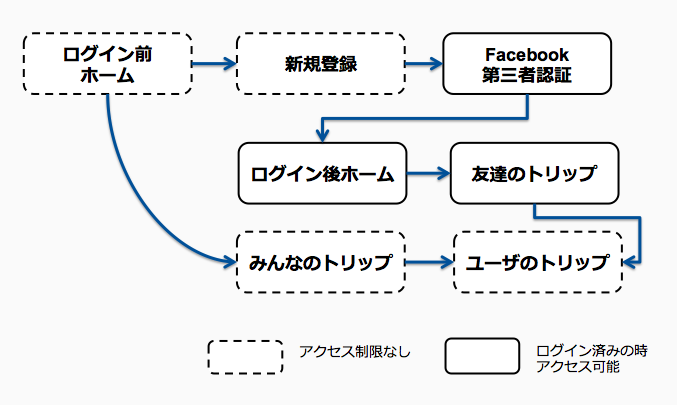
\includegraphics[width=12.0cm]{./image/cheekitrip_flow_screen.png}
\caption{画面遷移図}
\label{flow_screen}
\end{center}
\end{figure}


\subsubsection{ログイン前ホーム画面}

利用者が,本システムにはじめて訪れると「ログイン前ホーム画面」が表示される.この画面では,本システムの目的,機能を利用者に伝えている.

画面例を図\ref{screen_home_before_login}に示す.

\begin{figure}[!ht]
\begin{center}
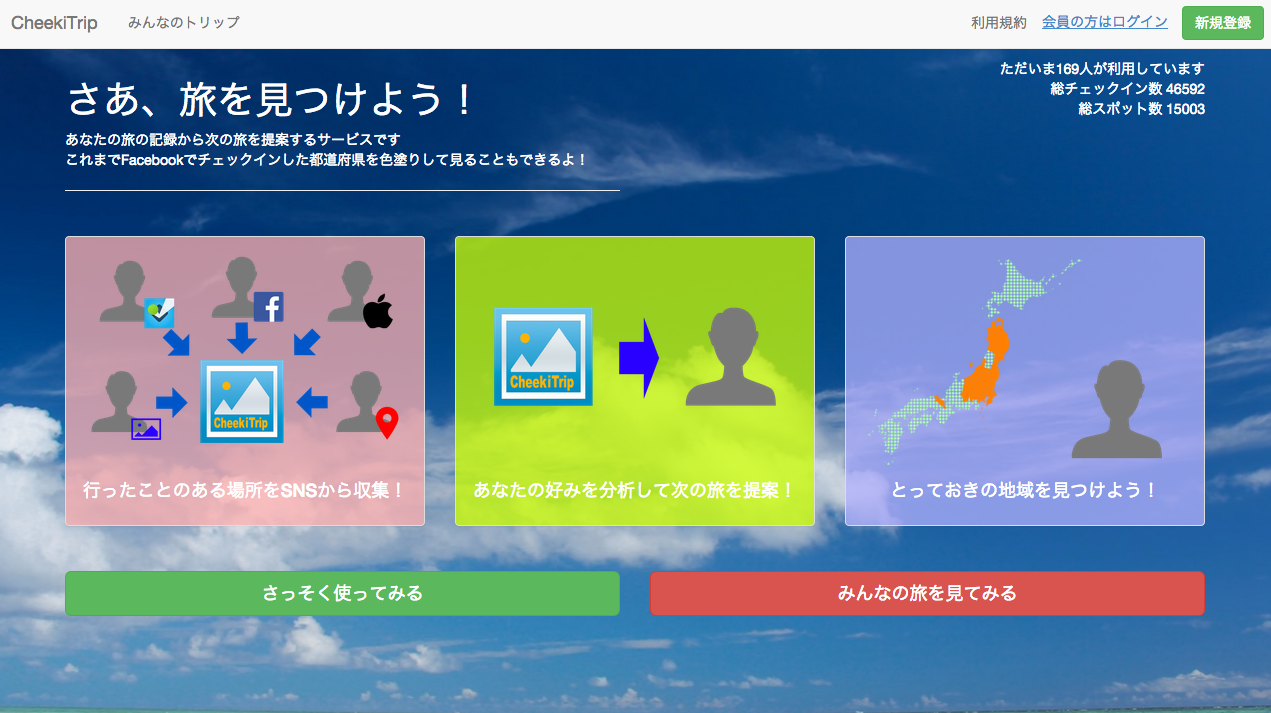
\includegraphics[width=12.0cm]{./image/cheektrip_top_before_login.png}
\caption{ログイン前ホーム画面}
\label{screen_home_before_login}
\end{center}
\end{figure}

\subsubsection{新規登録画面}

利用者がサービスを登録する,「新規登録画面」を用意した.

画面例を図\ref{screen_signup}に示す.

ここでは,利用規約やチェックインサービスで取得するデータを明確に示し,情報利用について承諾を得た上で利用してもらうことで,本システムの利用による倫理的な問題が起きないように配慮した.

\begin{figure}[!ht]
\begin{center}
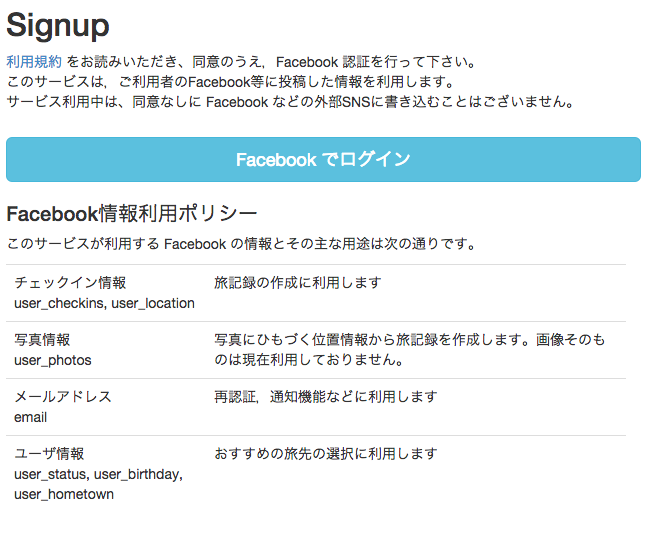
\includegraphics[width=15.0cm]{./image/cheekitrip_signup.png}
\caption{新規登録画面}
\label{screen_signup}
\end{center}
\end{figure}

\subsubsection{Facebook 第三者認証画面}

利用者に対して,本システムに対してデータ連携を許可を求めるダイアログが表示される設計とした.

画面例を図\ref{screen_auth_with_facebook}に示す.

利用者から許可を得た場合は,利用者のFacebook上のプロフィールおよびチェックインデータを本システムのデータベースに取り込むためにデーモンが起動する.

\begin{figure}[!ht]
\begin{center}
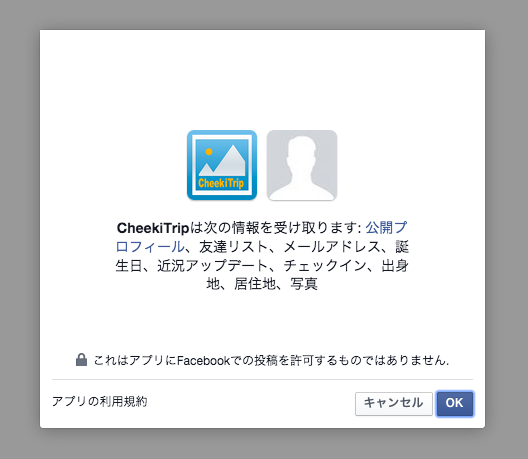
\includegraphics[width=12cm]{./image/cheekitrip_auth_with_facebook.png}
\caption{Facebook 第三者認証画面}
\label{screen_auth_with_facebook}
\end{center}
\end{figure}

\subsubsection{ログイン後ホーム画面}

ログインが完了した利用者向けのホーム画面を「ログイン後ホーム画面」と呼ぶ.この画面はダッシュボード型の画面になっており,利用者に向けて様々な情報が提示される.

画面例を図\ref{cheekitrip_home}に示す.

\begin{figure}[!ht]
\begin{center}
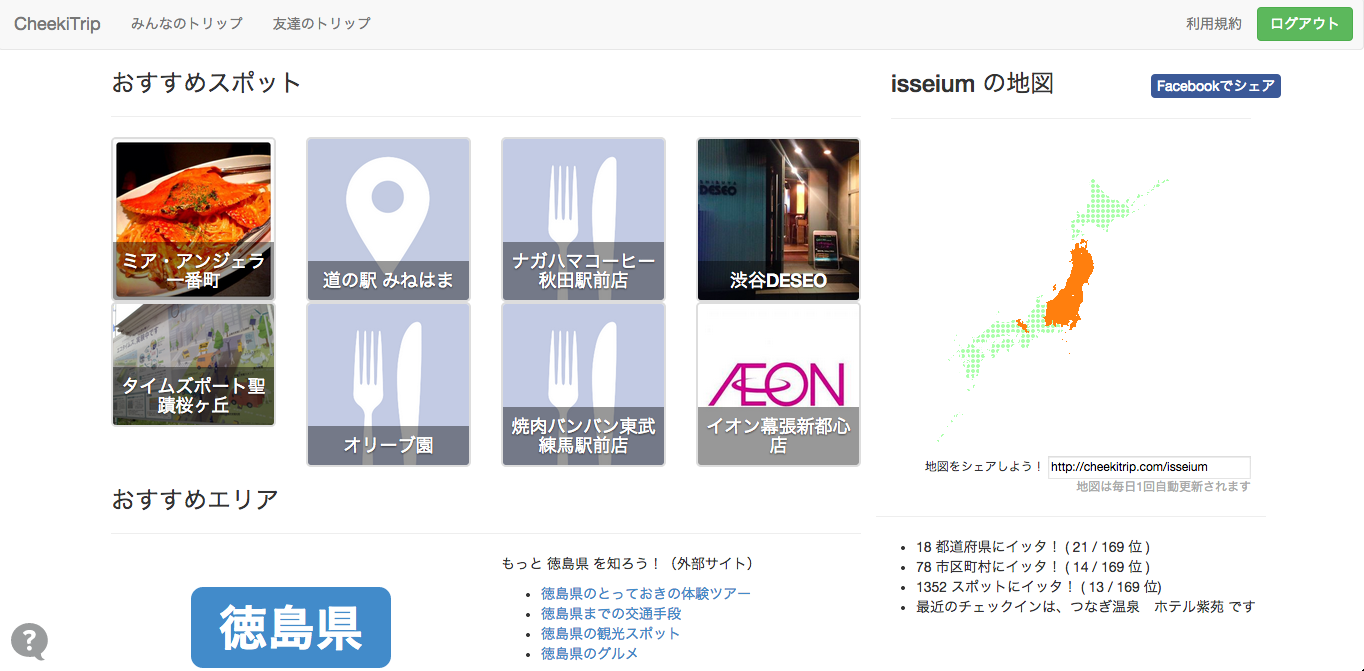
\includegraphics[width=12.0cm]{./image/cheekitrip_home.png}
\caption{ログイン後ホーム画面}
\label{cheekitrip_home}
\end{center}
\end{figure}

ログイン後ホーム画面に含まれる主な情報を説明する.

\begin{description}
\item[観光資源推薦情報] これまで訪れたことのある観光資源に基づいて推薦された観光資源.
\item[観光地域推薦情報] これまで訪れたことのある観光資源に基づいて推薦された観光地域(都道府県).併せて観光地域に関係する情報サイトへのリンクも掲載した.
\item[色塗り地図] これまで訪れたことのある都道府県を日本地図上で可視化した.訪れたことのある地域は朱色,訪れたことのない地域は緑色(水玉)で示した.
\item[シェア] 色塗り地図の画像をFacebookにシェアする.本機能によって,利用者間の競争意識を高め,本サービスの利用者促進を図った.
\item[統計情報] 自身のチェックインに関する統計情報を表示する.利用者内での自分の立ち位置がわかるランキング機能も備えた.
\item[友達に人気のスポット] 友達がよく行くスポットを表示する.(図\ref{cheekitrip_friends_popular_spot})
\item[友達が最近行ったスポット] 友達が最近行ったスポットを表示する.(図\ref{cheekitrip_friends_recently_spot})
\end{description}

\begin{figure}[!ht]
\begin{center}
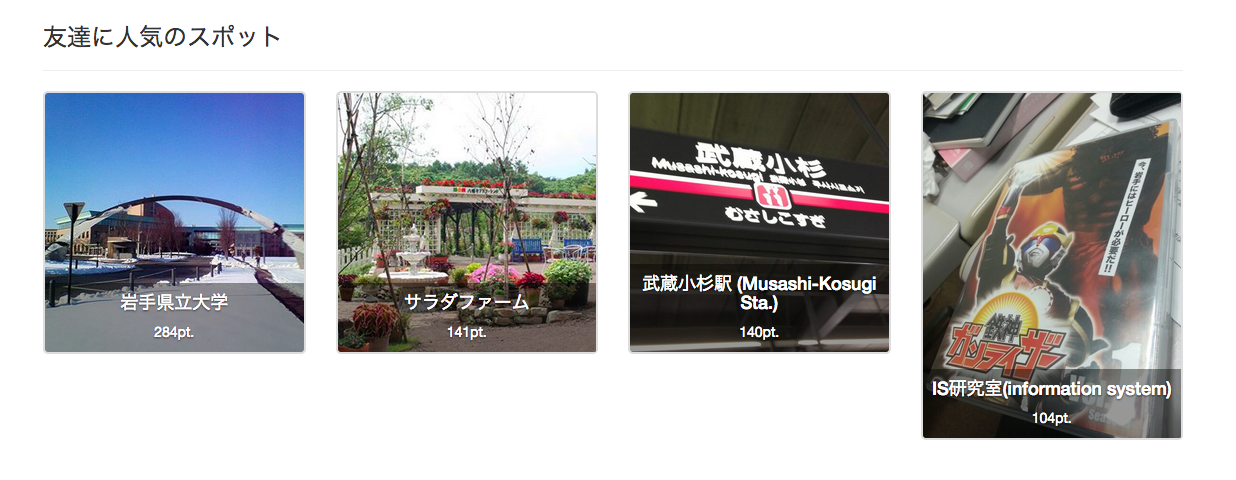
\includegraphics[width=12.0cm]{./image/cheekitrip_friends_popular_spot.png}
\caption{友達に人気のスポット}
\label{cheekitrip_friends_popular_spot}
\end{center}
\end{figure}

\begin{figure}[!ht]
\begin{center}
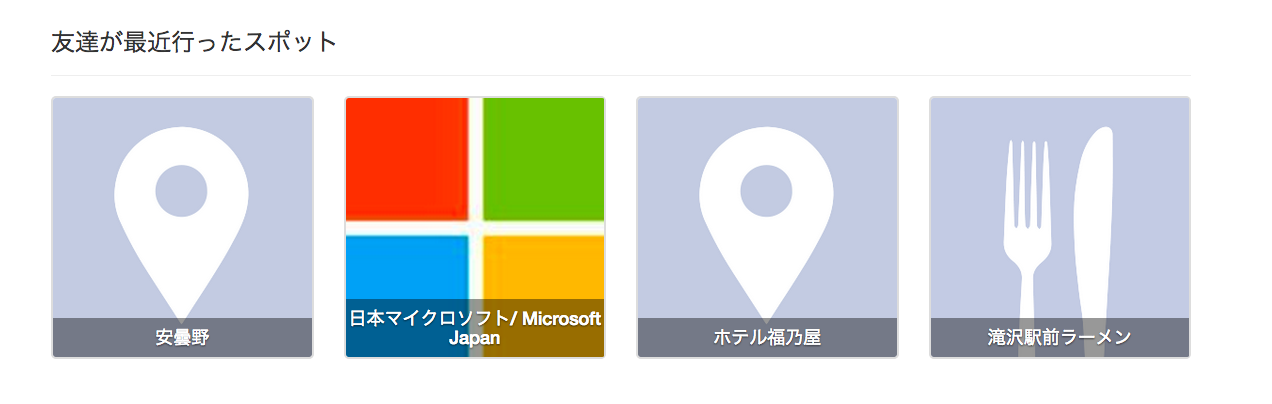
\includegraphics[width=12.0cm]{./image/cheekitrip_friends_recently_spot.png}
\caption{友達が最近行ったスポット}
\label{cheekitrip_friends_recently_spot}
\end{center}
\end{figure}

\subsubsection{みんなのトリップ画面}

本サービスの利用者全員のチェックインデータに基づく統計情報を示す画面である.
本画面では,利用者がよく訪問しているスポットを「みんなに人気のスポット」として表示している.

画面例を図\ref{cheekitrip_everyone}に示す.


\begin{figure}[!ht]
\begin{center}
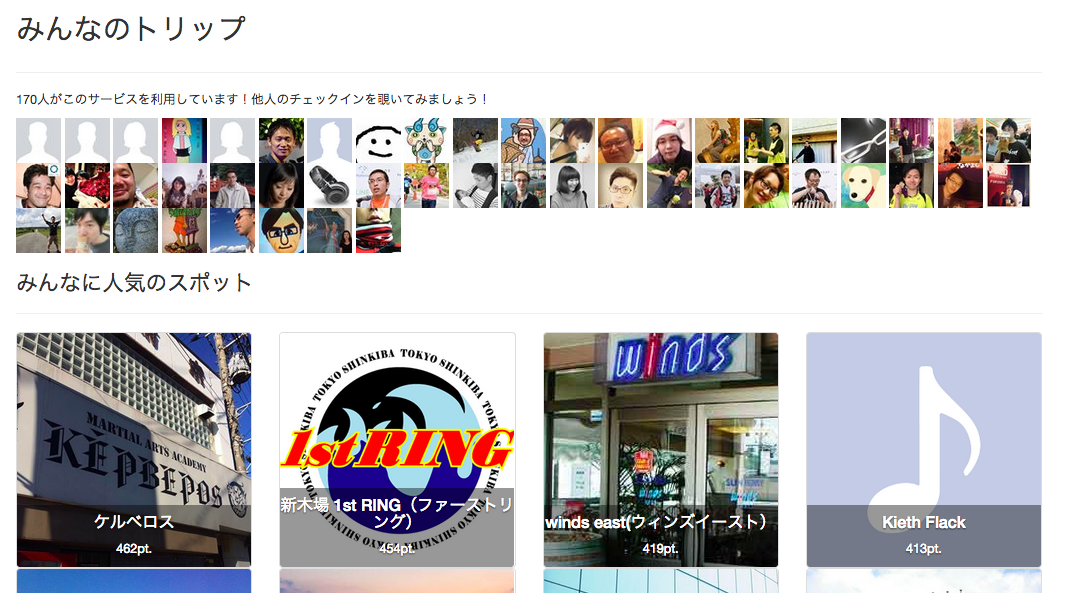
\includegraphics[width=12.0cm]{./image/cheekitrip_everyone.png}
\caption{みんなのトリップ画面}
\label{cheekitrip_everyone}
\end{center}
\end{figure}

\subsubsection{友達のトリップ画面}

利用者の友人の一覧を表示する画面である.本画面から友人のトリップ情報へのリンクをたどることができる.

画面例を図\ref{cheekitrip_friends}に示す.

\begin{figure}[!ht]
\begin{center}
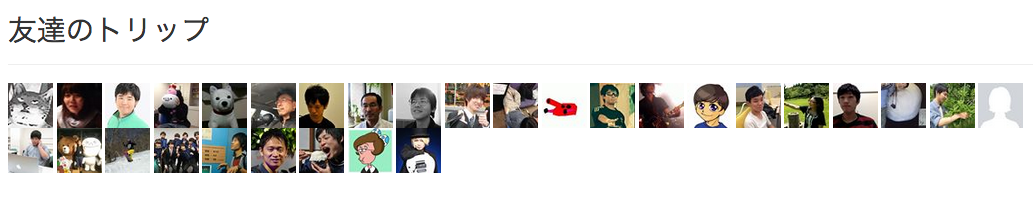
\includegraphics[width=12.0cm]{./image/cheekitrip_friends.png}
\caption{友達のトリップ画面}
\label{cheekitrip_friends}
\end{center}
\end{figure}

\subsubsection{ユーザのトリップ画面}

任意のユーザのチェックイン情報および推薦情報などが表示される画面である.原則として「ログイン後ホーム画面」と同様の情報が表示される.

\subsection{本章のまとめ}

本章では,研究の課題を解決するシステムの要件定義,設計,開発を行った.

要件定義では, 「利用者に手間をかけずに過去の観光行動を取得できること」および「実データを利用した推薦を実施し精度を評価すること」を挙げた.推薦精度の評価については,次章にて述べる.

設計では,利用者が多いチェックインサービスに着目し利用者の手間の軽減を図った.またApache Mahoutを利用することでプロトタイプ的に推薦を実施できるようにした. 工夫点としては,システム全体が取り扱うデータ量が多いことが想定されたため,データ特性に合わせたデータの管理およびシステム全体の設計としたことが挙げられる.


\newpage

\section{評価・考察}

行動データの観光推薦への活用可能性を検証することを目的として提案システムを開発し,実際にインターネット上に公開した.本章では,システム運用の概要および活用可能性の評価を行い,得られた知見をまとめる.

\subsection{システム運用の概要}

開発したシステムは,「CheekiTrip(チイキトリップ)」と名付けられ,2014年4月に一般公開された(http://cheekitrip.com).公開後は,クチコミ,オンライン広告などを利用して利用者の促進を図った.
システム運用の概要を表\ref{operation_description}に示す.また,サイト訪問者数の推移を図\ref{proc_users}に示す.


\begin{table}[!h]
\small
\caption{システム運用の概要(2014年7月27日現在)}
\begin{center}
\begin{tabular}{l|r}
\label{operation_description}
指標 & 値 \\ \hline
サービス開始日 & 2014年4月12日 \\
ページビュー & 5727PV \\
来訪ユニークユーザ & 732UU \\
登録ユーザ数 & 169人 \\
総チェックイン数 & 45506件 \\
総観光資源数 & 14575件 \\
推薦の閲覧数 & 1446回 \\
\end{tabular}
\end{center}
\end{table}

\begin{figure}[!ht]
\begin{center}
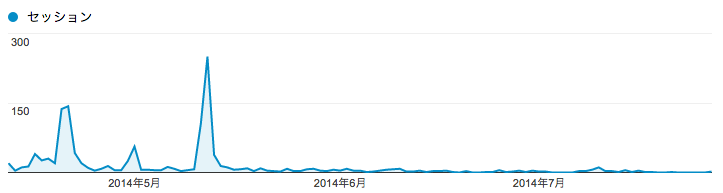
\includegraphics[width=15.0cm]{./image/proc_users.png}
\caption{サイト訪問者数の推移}
\label{proc_users}
\end{center}
\end{figure}
    
日本全体のチェックインの傾向を視覚的に表したヒートマップを図\ref{heatmap1}に示す.
主観的な考察であるが,日本各地にチェックインした行動データが収集されていることがわかる.

\begin{figure}[!ht]
\begin{center}
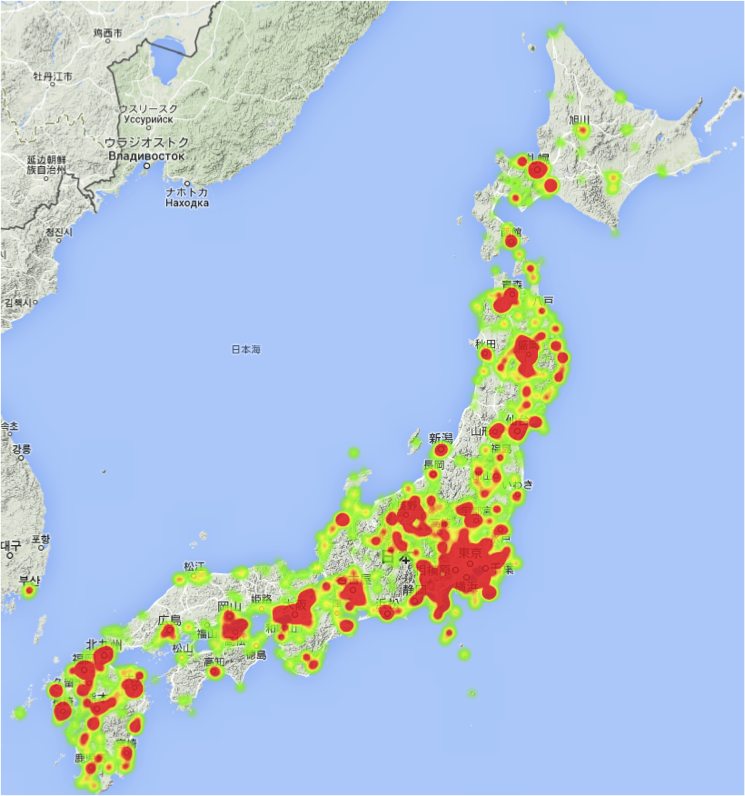
\includegraphics[width=8.0cm]{./image/heatmap1.png}
\caption{日本全体のチェックインヒートマップ}
\label{heatmap1}
\end{center}
\end{figure}

盛岡市のチェックインの傾向を視覚的に表したヒートマップを図\ref{heatmap2}に示す.主観的な考察であるが,盛岡市内の人が集まる観光資源へのチェックインが多いことがわかる.例えば,左部の領域は「小岩井農場」であり,右下部の領域は「盛岡駅」「大通り」などの商業エリアである.

\begin{figure}[!ht]
\begin{center}
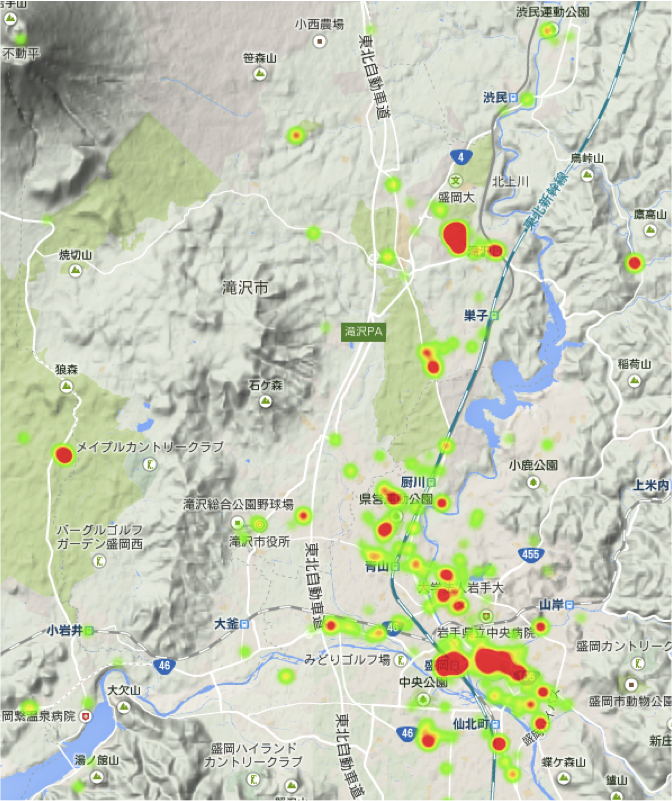
\includegraphics[width=8.0cm]{./image/heatmap2.png}
\caption{盛岡市のチェックインヒートマップ}
\label{heatmap2}
\end{center}
\end{figure}

\clearpage

\subsection{利用者からの評価(質的評価)}

本節では,開発したシステムの操作性と実用可能性について質的評価を行う.評価アプローチとしては,利用者へのインタビューとした.
利用者の一部に口頭でシステムに関してインタビューを行った.

インタビュー対象者の属性を表\ref{attribute_interview}に示す.

\begin{table}[ht!]
\small
\caption{インタビュー対象者の属性}
\begin{center}
\begin{tabular}{l|lllll}
\label{attribute_interview}
対象者ID & 性別 & 年齢 & 居住地 & 出身地 & 職業 \\ \hline
A      & 男性 & 21歳 & 岩手県滝沢市 & 青森県弘前市 & 学生 \\
B      & 男性 & 22歳 & 岩手県滝沢市 & 秋田県横手市 & 学生 \\
C      & 女性 & 20歳 & 岩手県滝沢市 & 秋田県潟上市 & 学生 \\
D      & 男性 & 22歳 & 岩手県盛岡市 & 岩手県盛岡市 & 学生 \\
\end{tabular}
\end{center}
\end{table}

\subsubsection{インタビューの観点}

インタビューでは,ある事象について振り返り,評価を行う「KPT法」を参考に下記の3つの観点を意識した.

\begin{description}
\item[よかった点,有用と感じたこと(Keep)] 
\item[悪かった点,使いにくいと感じたこと・課題と感じたこと(Problem)] 
\item[将来的に実現して欲しい機能や使い方(Try)] 
\end{description}

次小節以降では,インタビューの結果を3つの観点ごとに示す.

\subsubsection{Keepの観点からの評価}

Keepの観点から得られたインタビューの結果を示す.( )内は対象者IDである.

\begin{itemize}
\item オススメのスポットの画像がイメージしやすい (A)
\item 友達にとって人気のスポットがみれて参考にできそう (A)
\item 会員登録で Facebook 認証は便利だった (A)
\item 地図や統計情報から自分の履歴がみれるのがよい (C)
\item 色塗り地図によって自分がどこにいったかわかりやすい (D)
\end{itemize}

以上の結果を分析し,利用者の感想を次の2点に集約した.

\begin{description}
\item[色塗り地図に価値を持っている] 観光行動を振り返るサービスとして色塗り地図がよいという声が聞かれた.
\item[個人化推薦についての言及はない] いわゆる非個人化推薦である人気スポットの推薦については良好な意見があったが,個人化推薦について特に言及されることはなかった.
\end{description}

\subsubsection{Problemの観点からの評価}

Problemの観点から得られたインタビューの結果を示す.( )内は対象者IDである.

\begin{itemize}
\item どのように操作したら行ったことになるかわかりにくい (A, B)
\item おすすめの地域に偏りがある (A)
\item いきたいところない (A, B)
\item 既に行ったことのあるところが多い (B)
\item Facebook をあまりつかってない (C)
\item 推薦されたお店の写真が「行きたい」と言う気持ちにさせない (D)
\end{itemize}

以上の結果を分析し,利用者の考える課題を次の3つの問題とした.

\begin{description}
\item[システムの操作性の問題] 利用者の入力負荷軽減を狙ったシステムであるが,入力がほとんどないことで逆にシステム自体がなにをするものかわかりにくいという意見が聞かれた.
\item[推薦アルゴリズムに問題] すでに行ったところが推薦されていたことが要因で,「行きたいところがない」という意見が聞かれた.
\item[推薦結果の見せ方の問題] 推薦されたアイテムによっては,画像がなかったり視覚的に訴えるものがなかった.
\end{description}

\subsubsection{Tryの観点からの評価}

Tryの観点から得られたインタビューの結果を示す.( )内は対象者IDである.

\begin{itemize}
\item チェックインしなくても行ったことを検知してほしい (A)
\item 交通情報があるとよい (A)
\item ジャンル別に推薦されるとうれしい (B)
\item 順位の詳細なランキングがみたい (B)
\item スポットの紹介文がほしい (B)
\item Facebook 以外のデータ抽出 (C)
\item 友達のなかで自分がどのくらいの順位か気になる (D)
\item ログイン後もトップページあったほうがよい (D)
\item 「いった」「いきたい」の評価をシステムからしたい (D)
\item おすすめ度 (D)
\end{itemize}

以上の結果を分析し,利用者が求める新しい施策として次の3つに集約した.

\begin{description}
\item[チェックインサービス以外の自動収集の仕組み] チェックインサービスだけでは利用者の行動を捉えるのは不十分であり,別サービスや手動での入力を行える仕組みにニーズがある.
\item[画像以外の推薦結果情報] 現行のサービスでは,推薦結果は推薦したアイテム名と関連画像のみを利用者に示しているが,スポットの紹介文やジャンルなどのより詳細な情報も一度に閲覧したいというニーズがある.
\item[ランキングの充実] 友人やシステム利用者全体と比べて自分の観光行動がどのような位置づけにあるか把握したいというニーズがある.
\end{description}

\subsection{推薦精度の評価(量的評価)}

本節では,得られたデータを用いて推薦精度の量的評価を行う.評価アプローチとしては,「各ユーザの観光をどれだけ推測することができたか」という視点で交差検証することとした.評価指標としては,適合率,再現率,f値である.

交差検証を行うには,得られたデータを訓練データと正解データに分割する必要がある.分割には,以下の2つの視点でグループ化することにした.

\begin{enumerate}
\item 月単位の分割: 得られたチェックインデータをいったん月単位で分割し,該当月と該当外の月で交差検証を実施する.2011年8月から2014年7月まで36グループの評価指標を算出する.
\item 地域単位の分割: 得られたチェックインデータを都道府県単位で分割し,該当都道府県の20\%(ランダム)と該当外の都道府県とで交差検証を各都道府県ごとに3回実施した平均を評価値とする.
\end{enumerate}

また,入力データおよび推薦アルゴリズムの条件を表\ref{recommendation_condition}に示す.

\begin{table}[ht!]
\small
\caption{入力データおよび推薦アルゴズムの条件}
\begin{center}
\begin{tabular}{ll}
\label{recommendation_condition}
条件項目    & 内容 \\ \hline
推薦方法    & アイテムベース推薦 \\
類似度      & コサイン類似度 \\
1ユーザあたりの最大推薦数 & 5 \\
\end{tabular}
\end{center}
\end{table}



\subsubsection{推薦精度の基準}

推薦アルゴリズムの評価を行うには,なんらかの推薦精度の基準が必要である.しかしながら,既存の観光推薦システムにおいては,実際の行動データを用いた評価をしている研究は見当たらない.

そこで,本研究では,乱数を利用したランダムに推薦をした場合(以下,ランダム推薦)の精度を求め,これを推薦精度の比較対象とした.
ランダム推薦の推薦精度を表\ref{result_random}に示す.

\begin{table}[ht!]
\small
\caption{ランダム推薦による推薦精度(100回試行した平均値)}
\begin{center}
\begin{tabular}{lrrrrrr}
\label{result_random}
推薦アイテムの種類\指標    & 適合率 & 再現率 & f値 \\ \hline
観光地域(都道府県)        & 3.374\% & 11.213\% & 0.062 \\
観光地(市区町村)          & 0.322\% &  0.578\% & 0.014 \\
観光資源(スポット)        & 0.039\% &  0.022\% & 0.003 \\
\end{tabular}
\end{center}
\end{table}

\subsubsection{月単位の分割による推薦精度の結果}

ここでは月単位の分割での交差検定の結果を考察する.月単位の分割の評価結果を表\ref{result_monthly}に示す.

\begin{table}[!h]
\small
\caption{月単位の分割による評価結果}
\begin{center}
\begin{tabular}{lrrrrrr}
\label{result_monthly}
推薦アイテムの種類\指標            & 平均適合率 & 平均再現率 & 平均f値 & 最大適合率 & 最大再現率 & 最大f値 \\ \hline
観光地域(都道府県)    & 0.558\% & 12.666\% & 0.013 & 0.015\% & 40.000\% & 0.028 \\
観光地(市区町村)      & 0.242\% &  1.165\% & 0.006 & 0.009\% &  4.348\% & 0.015 \\
観光資源(スポット)    & 0.105\% &  0.102\% & 0.002 & 0.004\% &  0.440\% & 0.005 \\
\end{tabular}
\end{center}
\end{table}

全体的な概観としてf値に注目したところ,ランダム推薦よりも数値が低く,推薦精度が悪いことがわかる.
この要因のひとつとして,協調フィルタリングおよび月単位の分割の特性上,月をまたいで2回以上訪れた観光地等は推薦されないことが推察される.すなわち,月単位の分割での評価は,いわゆるリピーターを無視するため低精度になる傾向にあることがわかる.言い換えると,観光推薦アルゴリズムにはリピーターを考慮する仕組みが必要である.

\subsubsection{地域単位の分割結果}

ここでは地域単位の分割での交差検定の結果を考察する.地域単位の分割の評価結果を表\ref{result_area}に示す.

\begin{table}[!h]
\small
\caption{地域単位の分割による評価結果}
\begin{center}
\begin{tabular}{lrrrrrr}
\label{result_area}
推薦アイテムの種類\指標            & 平均適合率 & 平均再現率 & 平均f値 & 最大適合率 & 最大再現率 & 最大f値 \\ \hline
観光地域(都道府県)    & 2.962\% & 14.743\% & 0.113 & 20.000\% & 100.000\% & 0.333 \\
観光地(市区町村)      & 0.156\% &  0.451\% & 0.036 &  8.571\% &  37.500\% & 0.140 \\
観光資源(スポット)    & 0.009\% &  0.004\% & 0.001 &  0.597\% &   0.393\% & 0.005 \\
\end{tabular}
\end{center}
\end{table}

全体的な概観としてf値に注目したところ,ランダム推薦よりも数値が高く,推薦精度が高いことがわかる.
すなわち,地域単位での訪問の有無による協調フィルタリングによる観光推薦システムは,ランダムな推薦に比べて推薦精度が高く,今後の活用可能性があることが示唆された.

\subsection{本章のまとめ}

今回の実験では,実データを利用した協調フィルタリングによる観光推薦の適用可能性について評価した.
評価は,インタビューによる質的評価と機械学習領域で用いられる量的評価を行った.質的評価では,利用者にインタビューを実施し,本システムの有用性,課題,発展可能性を利用者から得た.他人の観光行動を閲覧することや自身の旅を振り返ることは有用であることがわかった.量的評価では,これまで実データを利用した観光推薦システムは見当たらなかったため,ランダム推薦を基準に比較をした.その結果,利用者がまだ訪れたことのない新しい地域への情報推薦の活用可能性が見えた.

現状,本システムはまだ実用可能段階ではないが,今後の改善のための利用者のニーズ,大量の観光行動データ,そして今後の改善評価を行うための評価軸や基準値を提示できた.本実験を通じて得た課題や気づきについては次章の「今後の展望」にて述べる.

\newpage
\section{おわりに}

本研究では, 行動データの観光推薦への活用可能性を検証することを目的として研究を進めた.
第1章では,本研究の概観として,観光の現状と推薦システムの現状を示した.
第2章では,本研究で扱う観光領域について調査し,本研究における観光の位置づけを述べた.
第3章では,観光領域での推薦システムの活用事例について調査し,本研究で解決を目指す具体的な課題を明らかにした.具体的には,データセットの問題,行動データ入力の問題,定量評価の問題を挙げた.
第4章では,課題解決を図った観光推薦システムの提案・設計を示した.課題を解決する要件として,利用者に手間をかけずに過去の観光行動を取得できることと,実データを利用した推薦を実施し,精度を評価できることを挙げた.
第5章では,開発したプロトタイプシステムの運用結果と質的評価および量的評価を実施した.

本章では,本研究のまとめとして結論を述べる.その後,今後解決していくべき課題や展望について述べる.

\newpage

\subsection{本研究の結論}

本研究の目的は,第3章において3つ掲げた.本節では,3つの課題それぞれに対して結論を述べる.また,本研究を通じて得られた知見等もまとめた今後の展望を述べる.

\subsubsection{データセットの問題に対する結論}

データセットの問題とは,推薦システムの研究の大きな動機付けである推薦精度向上のために必要なベースとなるデータセットが存在しないことに起因して,推薦精度向上を定量的に比較する方法がなかったことである.本研究では,現実世界の行動データのデータセットを収集することができたため,本問題を解決したと考える.

\subsubsection{行動データ入力の問題に対する結論}

行動データ入力の問題とは,推薦システムが必要とするユーザプロファイル(過去にどこへいったかなど)の入力は手間がかかることが予想され,簡略化の手法がなかったことである.本研究では,社会において利用者数の多いチェックインサービスの第三者利用の仕組みを活用することで,手間を掛けずにユーザプロファイルを収集することができたため,本問題を解決したと考える.

\subsubsection{行動データの定量評価に対する結論}
行動データの定量評価の問題とは,これまで観光推薦システムにおいて実際の行動データを利用した推薦精度の評価を実施した事例が見当たらなかったことである.本研究では,行動データを年月および地域別に交差検証し,推薦システムの精度指標である適合率,再現率,f値を求めることができたため,観光推薦領域において新しい視点での評価を行うことができた.

\subsection{今後の展望}

本節では,本研究を通じて得られた気づきや知見,課題を述べる.

\subsubsection{チェックインデータの分類(ノイズの除去)}

チェックインサービスから収集した行動データは,必ずしも観光行動のデータであるとは限らず,一般に観光行動以外のデータはノイズと考えられる.そのため,行動データを観光行動データと非観光行動データに分類するフィルタが必要と考える.具体的な手法としては,利用者の居住地(市区町村)でのチェックインや,居住地からの一定の距離内のチェックインを非観光行動とする方法がある.

一方で,非観光行動データから利用者の特性を見いだせる可能性もあるため,安易にノイズを削除するアプローチは好ましくないため注意を必要とする.

\subsubsection{チェックインデータ以外からの観光行動データの収集・活用}

チェックインサービスからの観光行動データだけでは不十分であり,別の自動収集もしくは手動入力の仕組みが必要である.
例えば,観光中にスマートフォンはデジタルカメラ写真を撮影することは多い.そこでこれらの情報を利用者プロフィールとして利用出来ないか検討する.具体的には,利用者のスマートフォンに保存されている写真の対象や撮影場所,日時などを分析したうえで利用することを想定している.

また,チェックインデータの内容(緯度経度など)とチェックインデータ以外の内容を比較したときに,それぞれのデータの傾向が浮かび上がるかも確認する必要がある.

\subsubsection{プロフィールデータの活用}

本研究では,SNS上のプロフィールデータも収集しているが,推薦アルゴリズムへの利用はされていない.そのため,このプロフィールデータの活用が必要である.例えば,性別,年代別,出身地別といった指標などを推薦システムに対して活用する方法がある.

また,訪日外国人に対する観光支援の仕組みのニーズもあるため,出身国を考慮した推薦システムの検討も行いたい.

\subsubsection{推薦アルゴリズムの選定・改良}

本研究では,実装が容易な協調フィルタリングを推薦アルゴリズムとして採用したが精度はよいとは言えなかった.そこで他の手法や重み付きの協調フィルタリングなどを試作し,精度を改善していく必要がある.また,同じ観光地へ2回以上訪問するリピーターを考慮した推薦の仕組みも必要である.

\subsubsection{利用者満足度の考慮}

本研究では,推薦システムが推薦したアイテムに関する利用者のフィードバックを収集する仕組みがない.例えば,「行ってみたい」「興味がない」といったことを利用者が意思表示し,推薦精度の向上につながる仕組みが必要であると考える.

\subsubsection{システム利用率向上のための施策}

運用しているシステムは,アクティブなユーザ数が少ない.観光という非日常的に実施される領域のサービスであるため,妥当な数値は不明であるが,日常的に利用されるような取り組みが必要である.加えて,新たにユーザを獲得する施策の検討も必要である.

\subsubsection{観光関係者向けシステムの構築}

本研究では,地域を訪問する利用者(旅行客)に対してのみフォーカスされたシステムとなっており,受け入れる地域側での視点が考慮されていない.本研究で収集されるデータを活用することで,地域ごとの「興味を持つ利用者像」「該当地域と類似する地域」といった視点での情報提供・分析ができる可能性がある.

\subsection{本章のまとめ}

本研究では,行動データの観光推薦への活用可能性を検証することを目的として研究を進めた.
本研究によって,利用者の入力付加を軽減したうえで,観光行動のデータセットを収集する仕組みを構築することができた.また収集したデータを質的・量的なそれぞれの視点で評価したところ,質的評価においては,観光推薦システムのニーズがある可能性が示唆された.量的評価においては,ランダム推薦よりも推薦精度が高く,将来的に行動データを用いた観光推薦システムの活用可能性があることが明らかになった.

一方,質的評価,量的評価それぞれの観点からみても現時点の観光推薦システムは,実運用は難しい.そこで本研究を通じて得られた知見をもとに今後の展望をまとめた.

最後に,本研究による成果が将来的に観光推薦システムおよび観光業界の発展と地方の活性化に貢献できることを期待する.

\newpage

\section*{謝辞}

本研究を進めるにあたり多くの方に協力をいただいた.2年間の大学院生活で関ったすべての方に感謝したい.

特に主査である佐々木淳先生には,一連の研究活動のみならず,3年間の社会人経験ののちに大学院の門を再び叩いた私に対して多大な支援をいただいた.深く感謝したい.また菅原光政先生,阿部昭博先生には副査として研究の流れ,評価方法などを中心にご指導をいただき心より感謝している.

佐々木研究室の教員の皆様にも感謝している.高木正則先生には,研究の進め方,課題の決定などで有益な助言をいただきた.山田敬三先生には,推薦アルゴリズムをはじめとする理論的な研究・技術について丁寧にご指導いただいた.

また,佐々木研究室の先輩・同期・後輩には,参考になるコメントをたくさんいただいた.この場を借りて感謝の意を示したい.特に,奧津翔太氏,菅原遼介氏,中島裕聡氏には研究活動のみならず,多くの活動をともにし,私の大学院生活がより豊かになったと考えている.また,同じ研究チームとして研究を進めた咲山拓哉君,手塚祐樹君,高橋靜音さん,李爽さんの協力にも感謝している.研究チームのさらなる研究の発展を期待したい.

さらに,学部時代の同期である佐々木拓也君にはCheekiTripの利用者数獲得において多大な貢献があった.同様に朽木拓君にはサービス運用におけるアドバイスをいただいた。学部時代の後輩である伊藤貴之君には,提案システムの画面設計において貴重な協力をいただいた.学部時代の先輩である及川一樹氏,山下和彦氏には大規模データの取り扱いや機械学習に関するテクニカルなアドバイスをいただいた.この場を借りて感謝申し上げたい.

最後に,もう一度学問することを快く応援してくれた家族に感謝する.

\newpage

\section*{研究業績・講演等}

\subsection*{研究発表}

主著の研究業績には,○印を付与している.

\begin{itemize}
\item ○ 小松 一星, 山田敬三, 高木正則, 佐々木淳, チェックインサービスを利用した観光履歴収集システムの提案, 電子情報通信学会, 2014年総合大会講演論文集,(2014-03-18).
\item Jun Sasaki, Takuya Sakuyama, Shizune Takahashi, Issei Komatsu, Keizo Yamada, Masanori Takagi, Local-Charm-Content Delivering Model by Using Web Advertisement and SNS, The 8th International Conference on Advanced Information Technologies (AIT), No.221, (2014-04-19).
\item ○ 小松一星, 高橋靜音, 咲山拓也, 山田敬三, 高木正則, 佐々木淳, Web広告を用いたターゲットユーザ絞り込み方法の提案, 平成26年度電気関係学会東北支部連合大会, (2014-08-22).
\item 盛内大輔, 小松一星, 漆原翔也, 高橋靜音, 咲山拓也, 山田敬三, 高木正則, 佐々木淳, 宅地付農地を対象としたWeb広告配信実験における広告媒体の比較, 平成26年度電気関係学会東北支部連合大会, (2014-08-22).
\item 漆原翔也, 小松一星, 盛内大輔, 手塚祐樹, 山田敬三, 高木正則, 佐々木淳, 宅地付農地を対象とした魅力発信モデルの提案, 平成26年度電気関係学会東北支部連合大会, (2014-08-22).
\item ○ Issei KOMATSU, Keizo YAMADA, Masanori TAKAGI,  and Jun SASAKI, Strategy to Activate Rural Areas Using Web Advertising and Social Networks, SOMET 2014, (2014-09).
\item 手塚祐樹, 咲山拓哉, 小松一星, 山田敬三, 高木正則, 佐々木淳, ID3を用いた訪問者プロフィールからの観光特性分析手法の提案, 情報処理学会全国大会, (2015-03 予定).
\item 高橋靜音,小松一星, 山田敬三, 高木正則, 佐々木淳, SNSデータを用いた個別ユーザ適応型観光スポット表示システムの提案, 情報処理学会全国大会, (2015-03 予定).
\item 李爽, 高橋靜音,小松一星, 山田敬三, 高木正則, 佐々木淳, 写真共有サービスを用いた外国人向け観光スポット推薦システムの提案, 情報処理学会全国大会, (2015-03 予定).
\end{itemize}

\subsection*{PBL}

2013年度PBLにて副代表としてプロジェクト運営を実施した.

\begin{itemize}
\item 林貴史, 小松一星, 門脇裕, 米田大地, 手塚祐樹, 2013年度PBL2013-06 観光促進支援システム「滝沢トリップ」の構築・評価, (2014).
\end{itemize}

\subsection*{講演等}

\begin{itemize}
\item 小松一星, 米田大地, Titaniumの紹介, IISAテクニカルカンファレンス2013, 口頭発表, (2013-11-22).
\item 小松一星, 2013年につくったもの, デジコン産学フォーラム, 口頭発表, (2014-01-23).
\item いわて若者会議2014, トークセッション「若者文化について語ろう!」, 登壇, (2014-02-16).
\item 小松一星, 僕のやりたいこと, 滝沢市IPU第2イノベーションセンター開所記念講演会, 口頭発表, (2014-05-30).
\item 小松一星, 盛内大輔, 漆原翔也, 高橋靜音, 雫石プロジェクトの紹介, IISAテクニカルカンファレンス2014, 口頭発表, (2014-11-21).
\item 岩手県人口問題対策本部, 若者の活躍と支援に関する意見交換会, 登壇, (2014-12-15).
\end{itemize}

% \newpage
% 
% \part*{添付資料}
% 
% 本研究に関わる資料を添付する.添付資料の一覧を表\ref{appendix}に示す.
% なお,資料の一部は,印刷を前提としないWebサービス(Confluenceなど)で作成したものも含まれており,読みにくいものもあるため,該当資料のURLなども極力示すようにした.
% 
% 
% \begin{table}[!h]
% \small
% \caption{添付資料の一覧}
% \begin{center}
% \begin{tabular}{lll}
% \label{appendix}
% 資料名 & 概要 \\ \hline
% CheekiTrip プロジェクト概要 & 提案システム開発を進めるうえでの計画,設計などの概要を記載した資料 \\
% CheekiTrip 画面設計書 & CheekiTripのデータベース仕様を記載した資料 \\
% CheekiTrip データベース設計書 & CheekiTripのデータベース仕様を記載した資料 \\
% CheekiTrip API設計書 & CheekiTripのAPI仕様を記載した資料 \\
% CheekiTrip 利用規約 & CheekiTrip の利用規約 \\
% ランダム推薦の推薦精度 & \\
% 月単位分割による評価結果(観光地域推薦) & \\
% 月単位分割による評価結果(観光地推薦) & \\
% 月単位分割による評価結果(観光資源推薦) & \\
% 地域単位分割による評価結果(観光地域推薦) & \\
% 地域単位分割による評価結果(観光地推薦) & \\
% 地域単位分割による評価結果(観光資源推薦) & \\
% 利用者インタビュー票 & \\
% 
% \end{tabular}
% \end{center}
% \end{table}
% 
% \newpage

\newpage
% 参考文献

\begin{thebibliography}{report}
\bibitem{action_program_2014} 日本政府 観光立国推進閣僚会議, 観光立国実現に向けたアクション・プログラム2014, (2014).
\bibitem{nippon_sousei} 日本創世会議 「ストップ少子化・地域元気戦略」 (2014).
\bibitem{tourism_stat} 日本旅行業協会,数字が語る旅行業2014, (2014).
\bibitem{tourism_future} 加藤弘治, 観光ビジネス未来白書, (2013).
\bibitem{kanko_hakusho_2009} 国土交通省観光庁, 平成21年度版 観光白書, (2009).
\bibitem{kanko_hakusho_2010} 国土交通省観光庁, 平成22年度版 観光白書, (2010).
\bibitem{kanko_hakusho_2011} 国土交通省観光庁, 平成23年度版 観光白書, (2011).
\bibitem{kanko_hakusho_2012} 国土交通省観光庁, 平成24年度版 観光白書, (2012).
\bibitem{kanko_hakusho_2013} 国土交通省観光庁, 平成25年度版 観光白書, (2013).
\bibitem{kanko_hakusho_2014} 国土交通省観光庁, 平成26年度版 観光白書, (2014).
\bibitem{wakamono_shinko} 国土交通省観光庁, 若者旅行振興の必要性について, (2011).
\bibitem{define_of_recommendation_system} J. A. Konstan and J. Riedl. Recommender systems: Collaborating in commerce and communities. In Tutorial at ACM CHI2003, (2003).
\bibitem{kamishima_recommendation} 神嶌敏弘, 「推薦システムのアルゴリズム」, (2014).
\bibitem{information_overload} P. Maes. Agents that reduce work and information overload. Communications of ACM, Vol. 37, No. 7, pp. 30-40, (1994).
\bibitem{kanko_define} 今井
\bibitem{japanese_society_list} Hirokazu Kobayashi, "観光学術学会が発足!(2012/04/30投稿)", ツーリズムマーケティングのフィールドから, http://hirokazukobayashi.air-nifty.com/marketing/2012/04/post-8570.html, (2014/12/14 参照)
\bibitem{yokomizo_1998} 溝尾良隆, 「観光・観光資源・観光地の定義 」, 観光研究, Vol.9, No.2, p.36, (1998).
\bibitem{toshin_1995} 建設省観光政策審議会, 今後の観光政策の基本的な方向について(答申39号), (1995).
\bibitem{tourism_law_2007} 日本国, 観光立国推進基本法, (2007).
\bibitem{tourism_kensetsu_1974} 建設省道路局, 観光レクリエーション交通調査, (1974)
\bibitem{recommendation_type_of_personalize} J. Ben Schafer, J. A. Konstan, and J. Riedl. E-commerce recommendation applications. Data Mining and Knowledge Discovery, Vol. 5, pp. 115-153, (2001).
\bibitem{tarui} 樽井 勇之, 協調フィルタリングとコンテンツ分析を利用した観光地推薦手法の検討,上武大学紀要集2001, 第36号, pp.1-14, (2011).
\bibitem{ctplanner} 倉田陽平, 対話型観光プランニングシステムに向けて, 第18回地理情報システム学会学術大会, 地理情報システム学会講演論文集 18, (2009).
\bibitem{ctplanner2} 倉田陽平, 有馬貴之, 対話的旅行計画作成支援システムの実装と評価, 第25回日本観光研究学会全国大会, 日本観光研究学会全国大会学術論文集 25, pp.173-176, (2010).
\bibitem{ctplanner3} 倉田陽平, Web上での対話的な旅行プラン作成支援. 情報処理学会第74回全国大会, (2012年).
\bibitem{ctplanner3b} 倉田陽平, CT-Planer 3: Web上での対話的な旅行プラン作成支援, 観光科学研究 5, pp.159-165, (2012). 
\bibitem{ctplanner4} 旅行プラン作成支援ツールCT-Planner4の留学生を対象としたモニター調査, 観光情報学会第10回全国大会, pp.56-57, (2013).
\bibitem{ctplanner5} 倉田陽平, 原辰徳, インターネット上での対話的旅行プラン作成支援サービスとその展開可能性, サービス学会第2回国内大会, pp.191-194, (2014).
\bibitem{ctplanner_web} CT-Planner, http://ctplanner.jp/ctp5/
\end{thebibliography}



\end{document}
